\chapter{Unsupervised learning \& clustering}
\section{Introductie}
Algemeen gezien bouwen \emph{machine learning}-technieken een model op basis van een (voorbeeld)-dataset; waarbij het doel is om een structuur die in de dataset zit naar boven te brengen. Het kan zijn dat deze structuur al aangeduid wordt doordat de data gelabeld is, in dit geval spreken we van \emph{supervised learning}. Indien de data nog niet gelabeld is, dient een \emph{unsupervised learning}-techniek gebruikt te worden.

\section{Clustering}
\emph{Clustering} is een typische \emph{unsupervised learning}-techniek, waarbij \emph{similarity groups} of clusters worden gezocht. Dit zijn data-elementen welke (per cluster) onderling sterk op elkaar gelijken. De data is dus nog niet geclassificeerd; er zijn geen labels voorzien. 

Om elementen met elkaar te kunnen vergelijken is een \emph{distance}-functie nodig. Door te clusteren dienen dan twee parameters geoptimaliseerd te worden:

\begin{itemize}
\item \textbf{Interclusterafstand}: De afstand tussen elementen van verschillende clusters dient maximaal te zijn. 
\item \textbf{Intraclusterafstand}: De afstand tussen elementen van eenzelfde cluster dient minimaal te zijn.
\end{itemize}

Het spreekt voor zich dat deze parameters een maatstaaf zijn voor de kwaliteit van het resultaat. De \emph{distance}-functie heeft een invloed op dit resultaat, alsook het algoritme zelf. Ook speelt het mee hoe de clusters gevormd zijn.
%
\begin{figure}[h]
\centering
\caption{Een voorbeeld van 6 elementen die met een hi\"erarchisch clusteringsalgoritme gegroepeerd zijn. }
\label{figure:hierarchical_clustering}
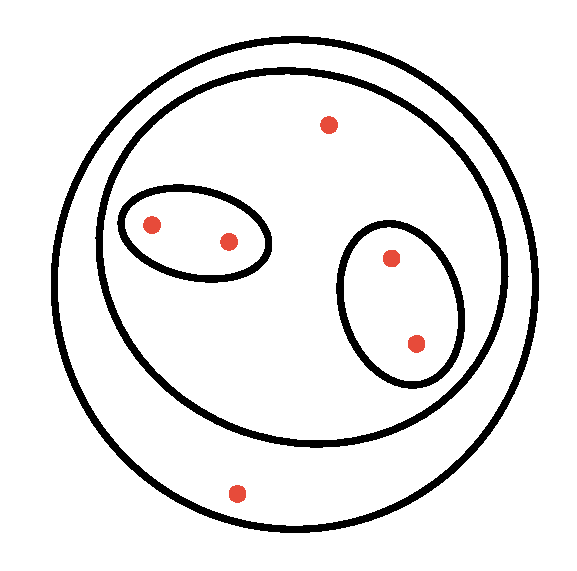
\includegraphics[width=0.40\textwidth]{res/ch4_hierarchical_clustering.eps}
\end{figure}
%
Wat algoritmes betreft, beschouwt men meestal twee soorten algoritmes. De eerste groep zijn de \emph{partitional clustering}-algoritmes, waar K-means onder valt. Hierbij wordt een groep elementen onderverdeeld in niet-overlappende subsets. \emph{Hierarchical clustering} is de tweede soort, waarbij een boomstructuur van geneste clusters wordt opgebouwd.  
%
\subsection{K-means}
Zoals eerder vermeld, is K-means een \emph{partitional clustering}-algoritme. De data wordt dus verdeeld in $k$ niet-overlappende clusters. Deze parameter $k$ wordt door de gebruiker opgegeven.

De data $D$ is een set van $r$ punten in een $n$-dimensionale vectorruimte. 

\begin{equation}
D= \{x_1, \dots, x_r \mid x_i \in \mathds{R}^n\}
\end{equation}

Elke cluster heeft een \emph{centroid}, een punt in het midden van de cluster. Bij de start van het algoritme worden $k$ punten random aangeduid als \emph{centroid}. Ieder punt wordt daarna een aan cluster toegewezen, afhankelijk van de afstand tot de \emph{centroid}. Hierna worden de \emph{centroids} herberekend, op basis van de huidige clusters. Dit wordt herhaald tot er geen convergentie meer waargenomen wordt. 

%%%%%%%%%%%%%%%%%%
% Indien dit gekopieerd wordt, zie: https://en.wikibooks.org/wiki/LaTeX/Algorithms
%%%%%%%%%%%%%%%%%%
\begin{algorithm}
\caption{Pseudocode voor het K-means-algoritme.}
\label{algo:kmeans}
\begin{algorithmic} 
\Require $k$: Number of clusters
\Require $D$: Data
\Function{k-means}{$k$,$D$}
    \State $C \gets randomSelection(k, D)$
    \Comment{Random centroids $C$}
    \Repeat
    \For {$x\in D$}
    	\For {$m \in C$}
        	\State compute distance from $x$ to $m$
        \EndFor
        \State assign $x$ to closest centroid $m$
    \EndFor
    \State $C \gets recomputeCentroids$
    \Until{stopping criterion is met}
    \State \Return $C$ 
\EndFunction
\end{algorithmic}
\end{algorithm}

Het \emph{stopping criterion} in algoritme \ref{algo:kmeans} kan op meerdere manieren ge\"implementeerd worden. Enkele mogelijkheden zijn:

\begin{enumerate}
\item Geen of weinig toekenningen van datapunten aan andere clusters.
\item Geen of minimale verandering van de \emph{centroids}.
\item Minimale afname in de \emph{sum of squared error}. Hierbij wordt per cluster $C_i$  de afstand $d$ tussen ieder punt $x \in C_i$ en de \emph{centroid} $m_i$ berekend.
\begin{equation}
SSE = \sum_{j=1}^k{\sum_{x\in C_i}{d\left( x, m_i \right)^2}}
\end{equation}
\end{enumerate}

\begin{figure}
\centering
\caption{Een voorbeeld van een gegenereerde tweedimensionale dataset, welke opgedeeld is in drie clusters van gelijke grootte.}
\label{figure:clusters}
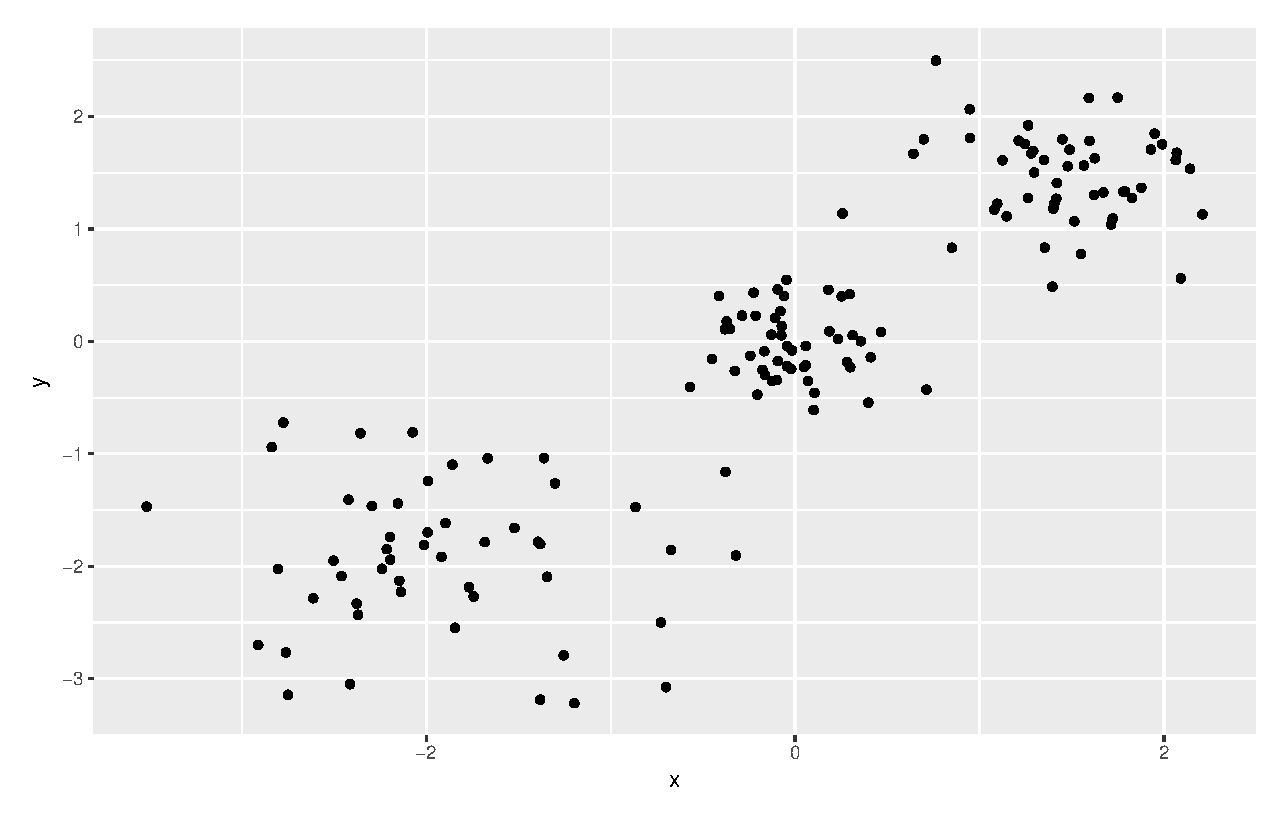
\includegraphics[width=\textwidth]{res/ch4_kmeans_before.eps}
\end{figure}

\begin{figure}
\centering
\caption{Op de dataset van figuur \ref{figure:clusters} is het \emph{K-means}-algoritme toegepast. De code voor het genereren van deze dataset en het clusteren staat op Github.}
\label{figure:clusters_kmeans}
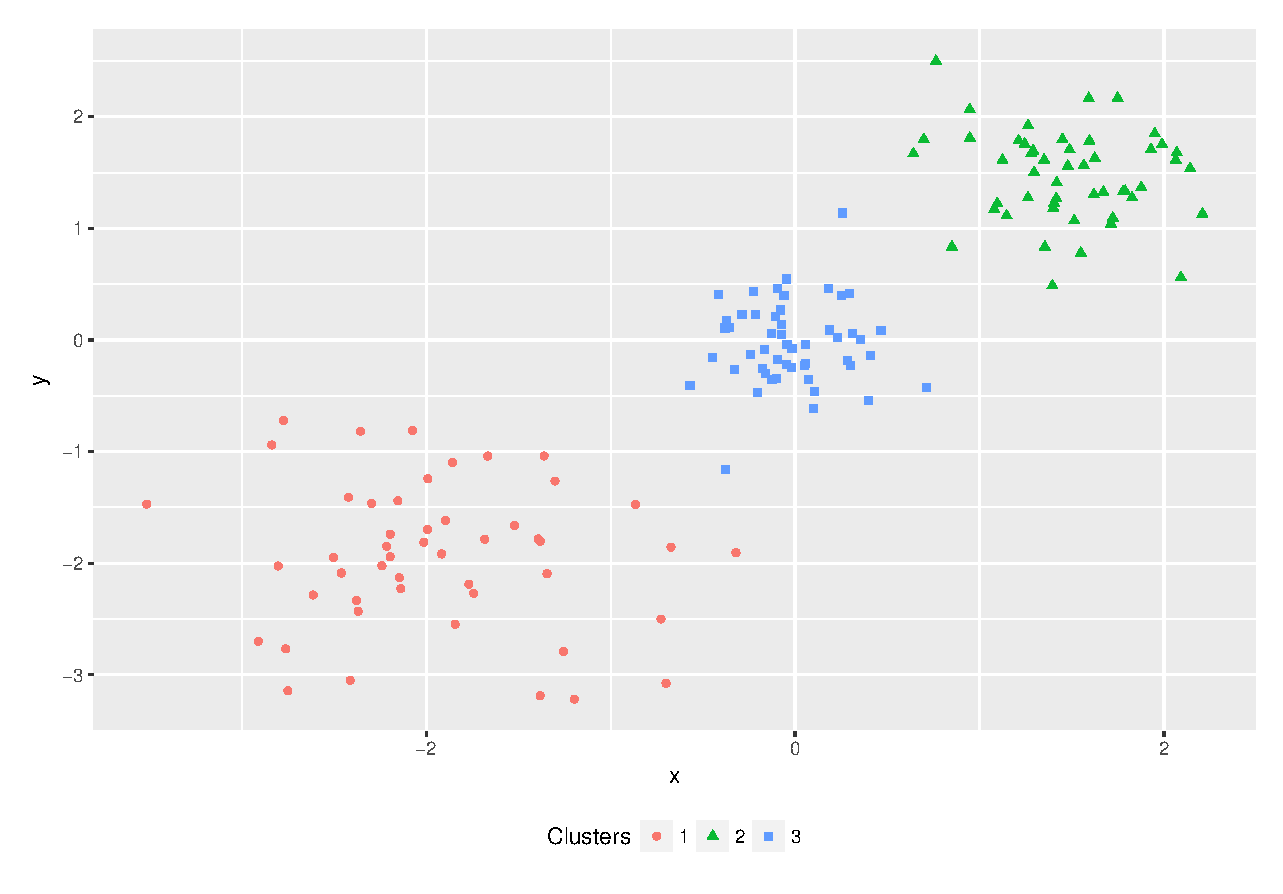
\includegraphics[width=\textwidth]{res/ch4_kmeans_after.eps}
\end{figure}

\paragraph{Distance functions}
In een Euclidische vectorruimte $\mathds{R}^n$ kan de afstandsfunctie $d$ op een volgende manier beschreven worden:

\begin{equation}
d(x,m)=||x-m||=\sqrt[]{\left(x_1-m_1\right)^2+\dots+\left(x_n-m_n\right)^2}
\end{equation}

Voor de \emph{centroids} is het dan mogelijk om het gemiddelde te gebruiken, wat per cluster $C_i$ tot de volgende formule leidt:

\begin{equation}
m_i^{t} = \frac{1}{|C_i^{t-1}|}\cdot \sum_{x\in C_i^{t-1}}{x}
\end{equation}

%
\paragraph{Voor- en nadelen}
Het K-means-algoritme is vrij eenvoudig om te begrijpen en te implementeren. Daarnaast is het ook nog behoorlijk effici\"ent, met een tijdscomplexiteit $O\left(k\cdot n \cdot i \cdot r \right)$ met $i$ iteraties \cite{jin2011k}. Er wordt ook veel werk gestoken in een paralleliseerbare versie \cite{zhao2009parallel}. Dit alles maakt dat K-means het populairste clusterings-algoritme is.

Er zijn echter ook nadelen aan het algoritme; waarvan de volgende het meest noemenswaardig zijn. 

\begin{itemize}
\item Het gemiddelde van een cluster dient gedefini\"eerd te zijn. 
\item Het algoritme is gevoelig voor initi\"ele \emph{centroids}; dit is ge\"ilustreerd in figuur \ref{figure:clusters_kmeans_wrong_seed}. Door meerdere \emph{passes} te doen, kan dit probleem verholpen worden. Daarnaast zijn er ook methoden om goede \emph{seeds} te kiezen voor de initi\"ele \emph{centroids}.

\begin{figure}
\centering
\caption{Dezelfde dataset van \ref{figure:clusters}, maar met ongelukkig gekozen \emph{centroids}. Merk op dat er nog steeds 3 clusters zijn, maar dat dit niet het globale optimum heeft gelokaliseerd. }
\label{figure:clusters_kmeans_wrong_seed}
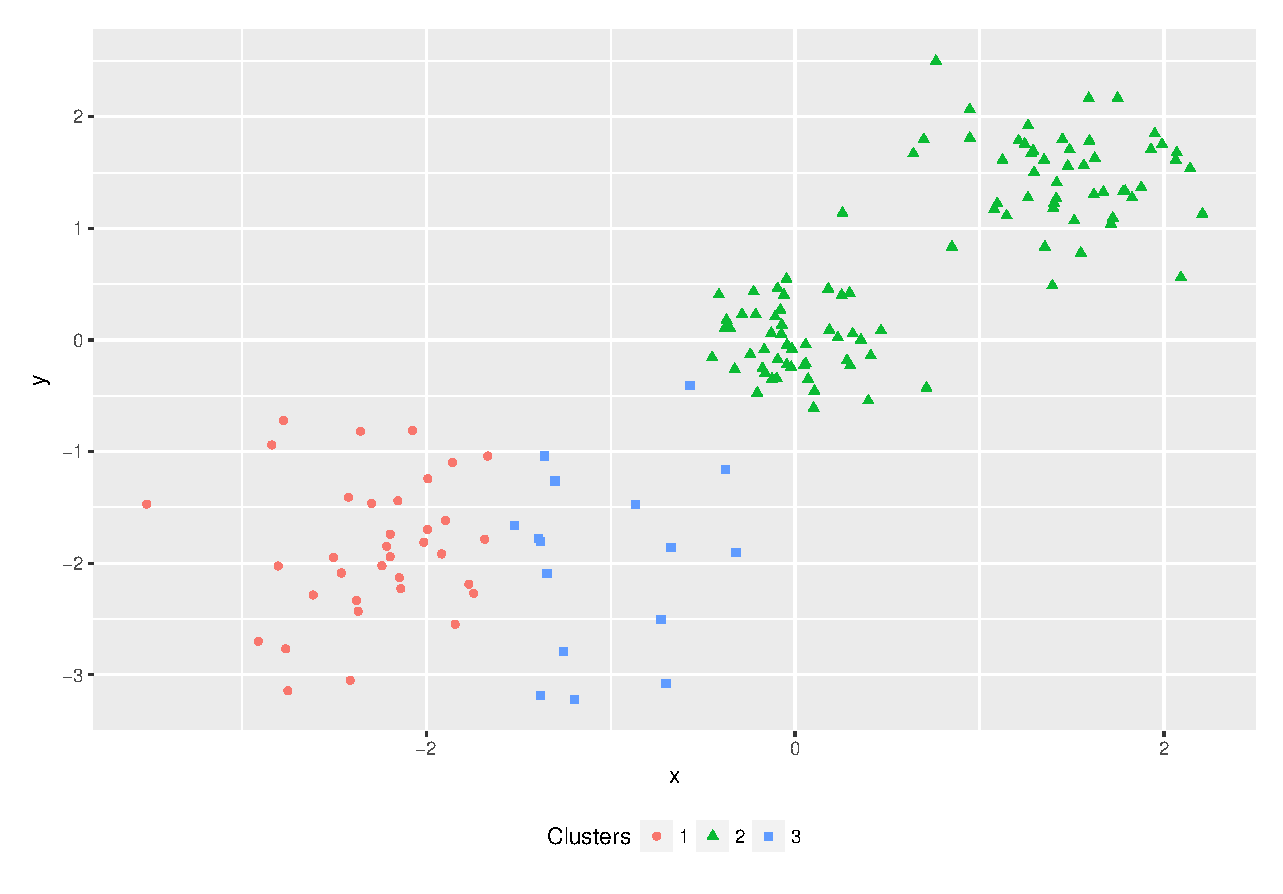
\includegraphics[width=\textwidth]{res/ch4_kmeans_wrong_seed.eps}
\end{figure}

\item De gebruiker dient zelf het aantal clusters $k$ op te geven.
\item Het algoritme is gevoelig voor \emph{outliers}. Dit kan opgelost worden door deze punten na enkele iteraties te verwijderen of door te clusteren op een random geselecteerde subset van de data. Dit verkleint de kans dat een \emph{outlier} geselecteerd wordt. 
\item K-means is enkel bruikbaar voor hyper-ellipso\"iden.


\begin{figure}
\centering
\caption{Een spiraalvormige dataset; nog steeds met 3 clusters. K-means is niet in staat de clusters correct te classificeren. De code hiervoor staat op Github.}
\label{figure:clusters_kmeans_spiral}
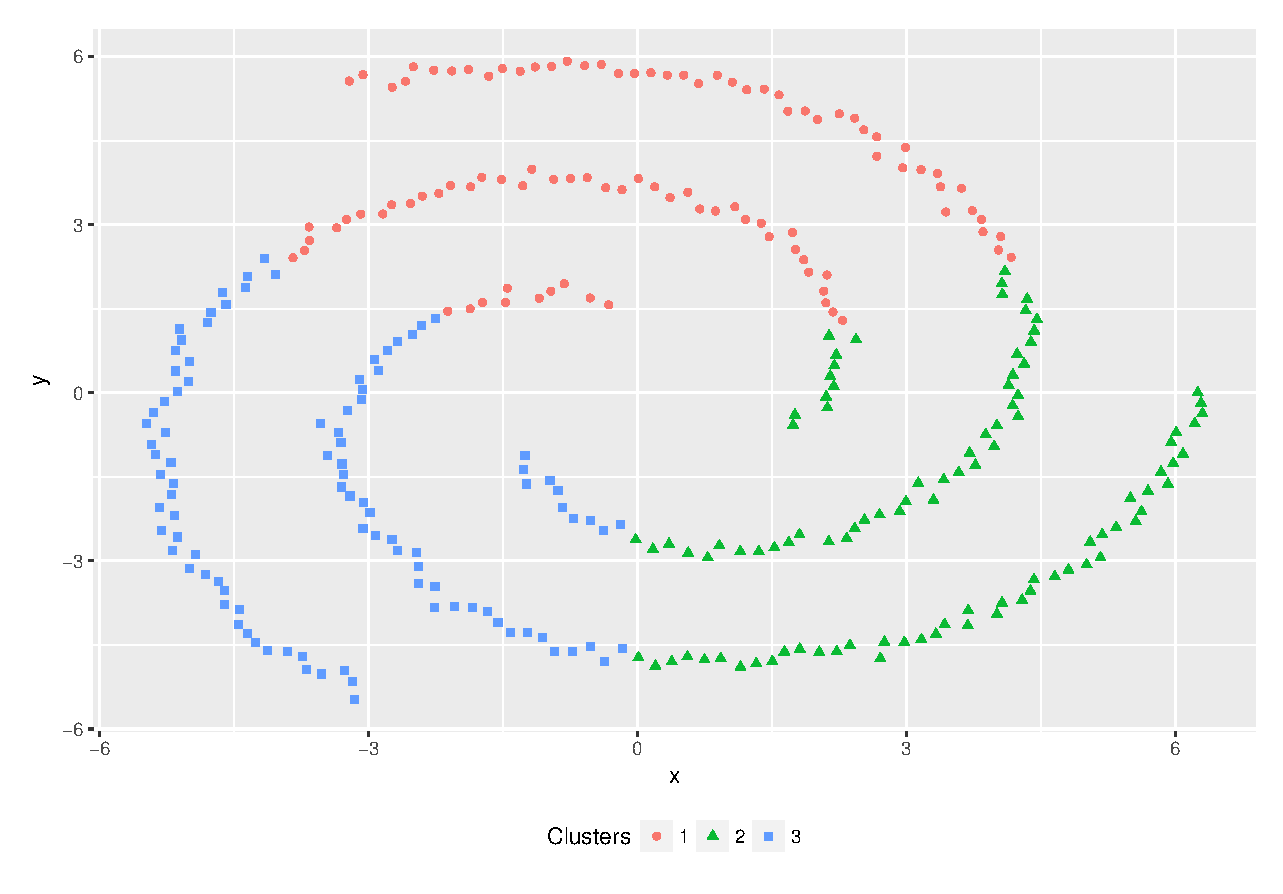
\includegraphics[width=\textwidth]{res/ch4_kmeans_spiral.eps}
\end{figure}
\end{itemize}
